\section{Метод конечных разностей для расчета токоперенос через гетероструктуру}
Конечно-разностная схема уравнения Шредингера (\ref{eq:ShredM}) для ГС на рис.\ref{fig:RTHSModel} \cite{Moskaluk}:
\begin{equation}
	\label{eq:ShFD}
	\psi_{i-1}\frac{m^{*}_{i+1}}{m^{*}_{i-1}} + \psi_{i}\bigg(  \frac{2\Delta^{2}m^{*}_{i+1}}{\hbar^{2}}(E-U_{i}) - \frac{m^{*}_{i+1}}{m^{*}_{i-1}} - 1 \bigg) + \psi_{i+1} = 0,
\end{equation}
\begin{conditions}
	$m^{*}_{i}$ & эффективная масса в точке $i$;\\
	$\psi_{i}$ & волновая функция в точке $i$;\\ 
	$E$ & энергия электрона;\\
	$U_{i}$ & потенциальная энергия в точке $i$;\\
	$\Delta$ & шаг сетки.
\end{conditions}

\begin{figure}
	\centering
	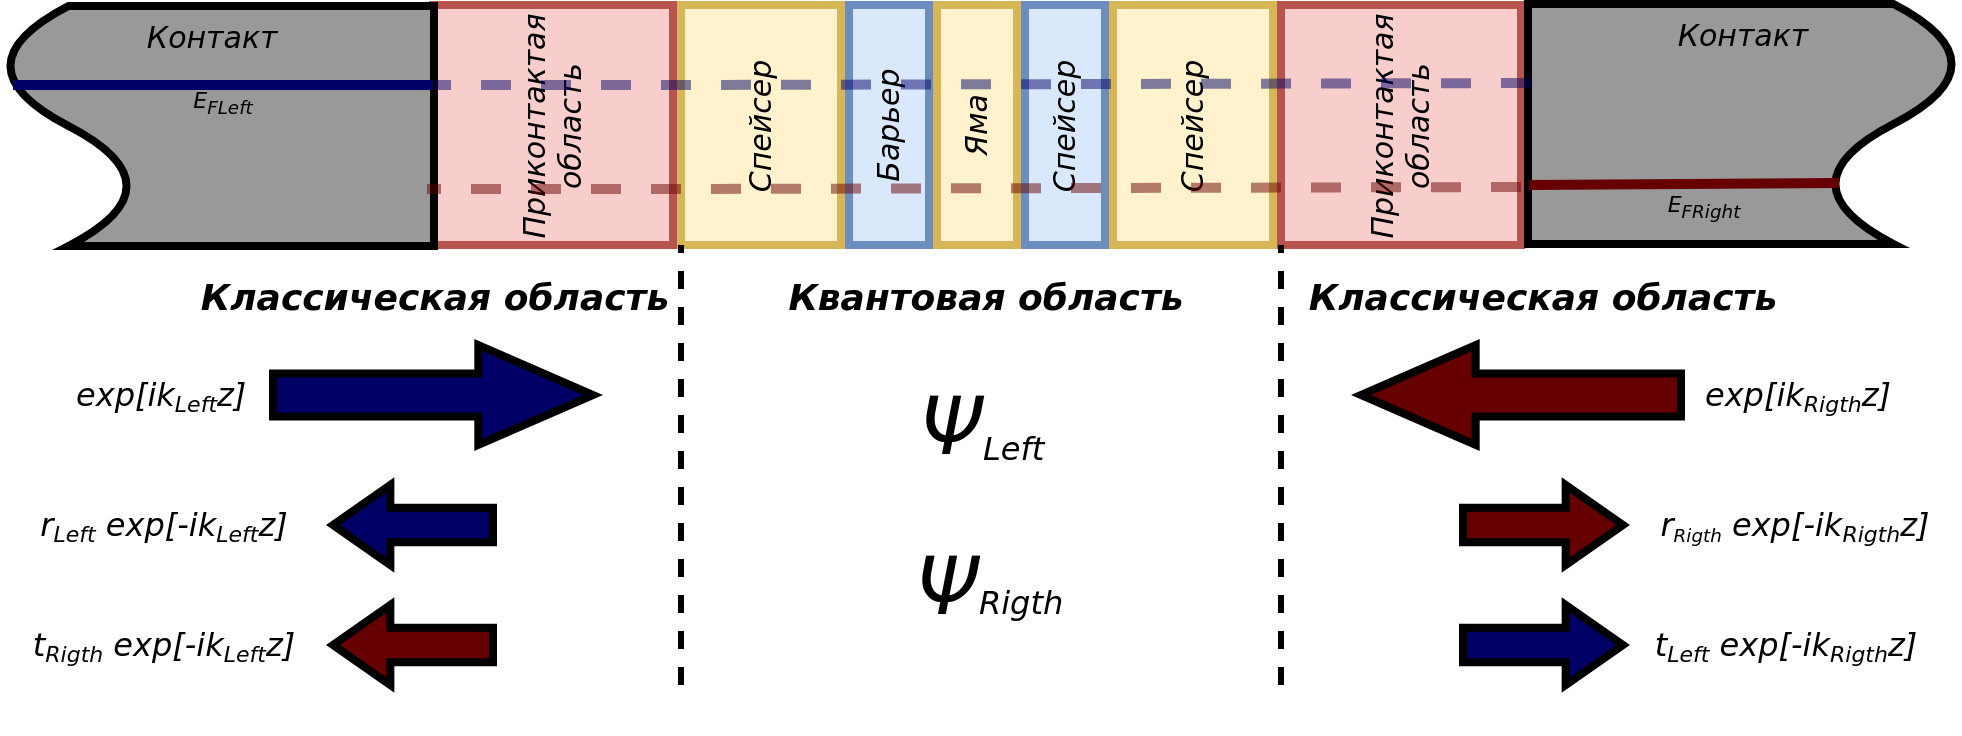
\includegraphics[width=1.08\linewidth]{RTHSModel}
	\caption{Схема модели РТГС}
	\label{fig:RTHSModel}
\end{figure}

Данное схема подходит для любой внутренней точки гетероструктуры, но не подходит для граничных точек. Граничные условия, для <<левых>> и <<правых>> электронов получаются из граничного условия Бастарда и вида волных функций в резервуарах:
\begin{gather}
	\label{eq:ShBound}
	\begin{cases}
		(ik_{L}-1)\psi_{1} + \psi_{2} = 2ik_{L}\Delta;\\
		\psi_{N-1} + (ik_{R}\Delta - 1)\psi_{N} = 0;
	\end{cases}\\
	\begin{cases}
		(ik_{L}-1)\psi_{1} + \psi_{2} = 2ik_{L}\Delta;\\
		\psi_{N-1} + (ik_{R}\Delta - 1)\psi_{N} = 0;
	\end{cases}
\end{gather}
\begin{conditions}
	$k_{L(R)}$ & волновые функции в левом (правом) резервуаре.
\end{conditions}

Для решения конечно-разностной схемы (\ref{eq:ShFD}), (\ref{eq:ShBound}) ур-ния Шредингера и получения волновых функций в среде \textsc{MatLab} была реализова функция \texttt{getWaveFunction} (лист.~\ref{lst:waveF}), которая находит решение уравнение Шредингера для элетронов из левого и правого резервуара.

Входными данными для данной функции являются: шаг сетки, сетка эффективной массы, сетка потенциального профиля, энергия электронов, для которой необходимо решить уравнение Шредингера. 

Выходными данными являются значения волновых функций с заданными энергиями в точках сетки.
\begin{lstlisting}[style=realcode,language=Matlab,caption={Решение уравнения Шредингера},label={lst:waveF}]
function [waveLeft, waveRigth] = getWaveFunction(delta, meff, U, Ez)
	hbar = 1.0551*1e-34;

	EzLen = length(Ez);
	ULen = length(U);

	waveLeft = zeros(EzLen, ULen);
	waveRigth = zeros(EzLen, ULen);

	for j = 1 : EzLen
		kLeft = sqrt( 2*meff(1)*(Ez(j) - U(1)) )/hbar;
		kRight = sqrt( 2*meff(end)*(Ez(j) - U(end)) )/hbar;

		d1 = ones(ULen-1, 1);
		d2 = 2*delta^2*meff(2:end-1).*( Ez(j)-U(2:end-1) )./hbar^2 - meff(2:end-1)./meff(3:end) - 1;
		d2 = [1i*kLeft*delta - 1, d2, 1i*kRight*delta - 1];
		d3 = [1, meff(2:end-1)./meff(3:end)];

		H = diag(d1, -1) + diag(d2) + diag(d3, +1);

		fLeft = [2*1i*kLeft*delta; zeros(ULen-1, 1)];
		fRight = [zeros(ULen-1, 1); 2*1i*kRight*delta];

		waveLeft(j, :) = (inv(H)*fLeft)';
		waveRigth(j, :) = (inv(H)*fRight)';
	end
	
end
\end{lstlisting}
В строке 2 вводится постоянная Дирака. В строках 4, 5 получают длину массива рассчитываемых энергий электрона и длина потенциального профиля. В строках 10-26 цикл рассчета волновых функций. В строках 7, 8 рассчитываются волновые вектора на <<левой>> и <<правой>> границах активная область -- резервуары. В строках 14-17 задается конечно-разностная (\ref{eq:ShFD}), (\ref{eq:ShBound}). В строке 19 создается матрица, соответствующая (\ref{eq:ShFD}), (\ref{eq:ShBound}). В строках 21, 22 задаются граничные условия для <<левых>> и <<правых>> электронов. В строках 24, 25 решается уравнение Шредингера для <<левых>> и <<правых>> электронов.

Для расчета плотности тока через ГС с помощью формулы Цу-Есаки (\ref{eq:J}) в среде \textsc{MatLab} была реализована функция \texttt{getJ} (лист.~\ref{lst:J}).

Входные данные: шаг сетки, сетка эффективной массы электрона, профиль дна зоны проводимости, прикладываемое к РТГС напряжение смещения, уровень Ферми в резервуарах.

Выходыне данные: Массив плотности тока через гетеро структуру при соответствующем смещении напряжения.

\begin{lstlisting}[style=realcode,language=Matlab,caption={Расчет плотности тока по формуле Цу-Есаки},label={lst:J}]
function J = getJ(dx, meff, Ec, dU, EFermi)
	e = 1.6e-19; eVtoJ = e; JtoEv = e^(-1); 
	hbar = 1.054*1e-34; k_B = 1.38e-23;

	T = 300;
	kT = T*k_B;

	k = ((2*meff(1)*e*kT)/(4*pi^2*hbar^3));
	J = k*ones(1, length(dU));

	for j = 1:length(dU)
		Uj = Ec - linspace( 0, dU(j), length(Ec) );
		dTDEz = @(Ez) TDEz(dx, meff, Uj, Ez, EFermi);
		J(j) = J(j)*integral(dTDEz, 0, max(Uj), 'AbsTol', 1e-35);
	end
end
\end{lstlisting}
В строке 2 задаются: заряд электрона и константы перевода из эВ в Дж и наоборот. В строке 3 задаются постоянная Дирака и константа Больцмана. В строках 5, 6 задаются температура системы и энергия тепловых колебаний. В строке 8 задается прединтегральный множитель формулы Цу-Есаки (\ref{eq:J}). В строках 11-15 расположен цикл расчета плотности тока при некотором смещение напряжения из массива входных данных. В строке 12 задается линейное падение напряжения на гетероструктуре. В строке 13 задаются входные данные функции \texttt{TDEz} (лист.~\ref{lst:TDEz}) для дальнейшего численного интегрирования. В строке 15 производится численное интегрирование по энергиям от 0 до максимального значения потенциальной энергии.

Для расчета численного расчета интеграла из формулы Цу-Есаки (\ref{eq:J}) в среде \textsc{MatLab} была реализована функция \texttt{TDEz} (лист.~\ref{lst:TDEz}).

Входные данные: шаг сетки, сетка эффективной массы электрона в зоне проводимости, сетка потенциальной энергии электрона, энергия электрона, для которой необходимо провести расчет, уровень Ферми в резервуарах.

Выходные данные: Функция возвращает подинтегральное выражение, которое затем стандартная функция в \textsc{MatLab} \texttt{integral} суммуриет и получает численное решение интеграла.

\begin{lstlisting}[style=realcode,language=Matlab,caption={Подъинтегральное выражение формулы Цу-Есаки (\ref{eq:J})},label={lst:TDEz}]
function val = TDEz(delta, meff, U, Ez, EFermi)
	hbar = 1.0551*1e-34; k_B = 1.38e-23;

	T = 300;
	kT = T*k_B;

	kLeft = abs( sqrt( 2*meff(1)*(Ez-U(1)) )/hbar );
	kRight = abs( sqrt( 2*meff(end)*(Ez-U(end)) )/hbar );

	[waveLeft, ~] = getWaveFunction(delta, meff, U, Ez);

	T = (kRight./kLeft).*(meff(1)/meff(end)).*(abs(waveLeft(:, end)).^2)';
	D = log( ( 1 + exp( (EFermi + U(1) - Ez)/kT ) ) ./ ( 1 + exp( (EFermi + U(end) - Ez)/kT ) ) );

	val = T.*D;
end
\end{lstlisting}
В строке 2 задаются постоянная Дирака и константа Больцмана. В строках 4, 5 задаются температура системы и энергия тепловых колебаний. В строках 7, 8 рассчитываются модули волновых векторов электрона на <<левой>> и <<правой>> границе активная область резервуары электронов. В строке 10 рассчитываются волные функции <<левых>> электрона, так как правыми можно принебречь в случае <<опускания>> потенциального рельефа справа. В строке 12 рассчитывается коэффицент прозрачности гетероструктуры, в соответствии с (\ref{eq:T}). В строке 13 рассчитывается функция снабжения электронами в соответствии с (\ref{eq:De}). В строке 15 проиходит поэлементное умножение рассчитанных значений.
